To exemplify a \emph{holistic test case} specification (see Section~\ref{subsec:testcasedescription}), an example is mapped to the holistic description:

\textbf{Narrative:} 
An aggregator, controlling DERs in 500 households, wishes to participate in the ancillary service markets by providing secondary frequency control to the transmission system operator (TSO). The presented example is a part of pre-qualification tests an aggregator must pass \cite{bondy2016procedure} in order to participate in aforementioned markets. Fig.~\ref{fig:examplediagram} presents the general system configuration. In this test case we analyse how the aggregator control system tracks the Automatic Generation Control (AGC) signal supplied by the TSO when subjected to disturbances in its ICT infrastructure. Metering issues and impact on the distribution grid are out of scope of this specific test. The holistic test case is described by:
\begin{itemize}
    \item \textbf{PoI:} to characterize the sensitivity towards ICT disturbances of the ancillary service quality of an aggregator.
    \item \textbf{SuT:} the system under test is composed of the aggregator infrastructure and 500 households. The input to the system is the AGC signal sent by the TSO and the output is the power consumption/production of the households.
    \begin{itemize}
    \item \textbf{OuI:} aggregator control system (part of the aggregator infrastructure).
    \item \textbf{DuI:} electric power and ICT infrastructure.
    \end{itemize}
    \item \textbf{FuT:} Aggregator central control, local DER control, communication functionality between aggregator and home energy management system (HEMS).
    \begin{itemize}
        \item \textbf{FuI:} Aggregator central control.
    \end{itemize}
    \item \textbf{Test Criteria:} 
    \begin{itemize}
        \item \emph{Target criteria:} Service quality, measured as the difference between the reference signal from the TSO and the aggregated power consumption/production of the DERs as measured by the individual DER measurement systems.
        \item \emph{Variability Attributes/Test Factors:} The ICT connection between aggregator and HEMS.%\bondy{based upon the discussion in the holistic testing group on May 31st, we seem to miss an explicit statement of where the variability in the test lies. Following the vocabulary from DoE I propose \emph{test factors}}
        %\kh{sounds good, though, well, in parallel, i suggested the terms in section III.B -- on the one hand I'd like to avoid DoE vocabulary overlap, as it first comes in at 'Mapping', but on the other, i also like my own suggestions :P}
        \item \emph{Quality Attributes/thresholds:} The ICT parameters are to be varied until the aggregator is unable to track the AGC according to the contract.
    \end{itemize}
\end{itemize}

\begin{figure}[!t]
\centering
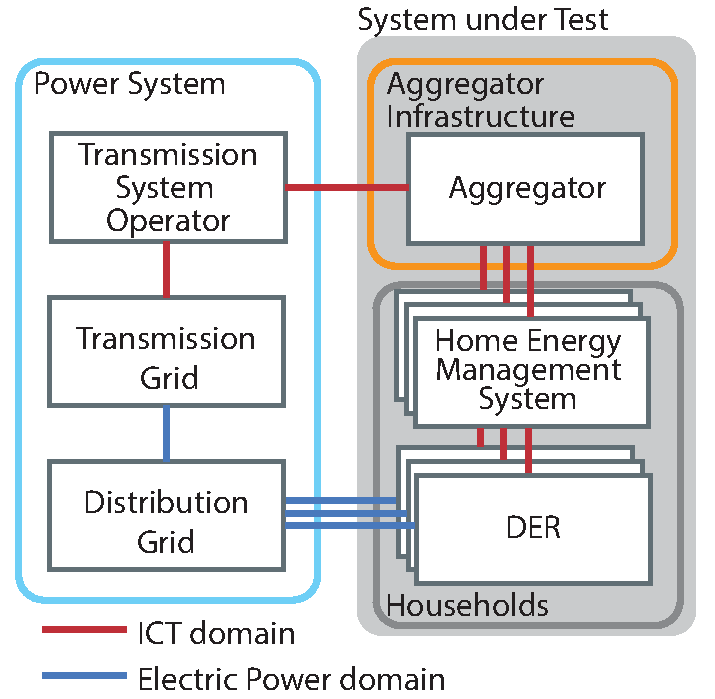
\includegraphics[width=0.75\columnwidth]{figures/example_diagram1.pdf}
\caption{The test setup described by the component centric approach. Note that the aggregator infrastructure and households form the \textbf{SuT}.}% 
\label{fig:examplediagram}
\end{figure}

A sub-test could be a set of physical tests for an aggregator--single household setup, which has as outcome an availability/disturbance model to be used in another (simulation) test setup including a 500 household controller hardware-in-the-loop simulation.